\documentclass[11pt,a4paper]{article}
\usepackage[margin=2.4cm]{geometry}
\usepackage{microtype}
\usepackage{amsmath}
\usepackage{booktabs}
\usepackage{graphicx}
\usepackage[font=small]{caption}
\usepackage[hidelinks]{hyperref}

\title{Detecting backdoor inferences from hardware performance counters}
\author{Nishanth D'souza\\[2pt] \small IITK Round One, Problem 1}
\date{October 2026}

\begin{document}
\maketitle

\begin{abstract}
\noindent
We are given 800 hardware performance counter (HPC) traces of clean neural-network inferences and asked to detect
backdoor-triggered inferences in a hidden test set. With no backdoor examples to learn from, we model the clean
traces with a three-component Gaussian mixture and flag traces that have low likelihood under it. The threshold is
calibrated on held-out clean traces for a 10\% false-positive rate. On public traces with real backdoor labels from
Alam et al.~\cite{alam2024}, the same procedure reaches an AUROC of 0.87, while detectors that treat clean data as
one cluster are at chance.
\end{abstract}

\section{Problem}

Each trace holds three counters measured during one inference: cache-references, cycles and LLC-loads. The
training file contains only clean inferences. The test set contains clean and backdoor inferences, and is scored on
accuracy, TPR, FPR, F1 and AUROC. This makes the task novelty detection: we need a score for how unlike the clean
traces a new trace is, and a threshold on that score.

The reasoning, following Alam et al.~\cite{alam2024}, is that a triggered input can change how the network uses
the cache and how long it runs, and that the change shows up in the counters. It does not have to. A trigger can
leave the counters exactly where clean inputs put them, and Section~\ref{sec:limits} comes back to this.

\section{The clean data}

The file has 800 rows, no missing values and no duplicate rows. Cache-references and LLC-loads are strongly
correlated (Pearson $r = 0.92$), and each is moderately correlated with cycles ($0.53$ and $0.54$). After
standardising, the first two principal components hold 78.1\% and 19.2\% of the variance. The third holds 2.7\%
and is essentially LLC-loads minus cache-references.

The traces sit in two groups along the cache-references/LLC-loads line, with 572 and 228 traces
(Figure~\ref{fig:data}). The split is stable under bootstrap resampling (adjusted Rand index 0.94). We do not know
what separates the groups. In the public data of Alam et al., similar groups followed the order in which traces
were recorded, but here no counter trends with row order ($|\rho| < 0.04$).

Cycles has a long right tail (excess kurtosis 6.8) that comes from three traces. The largest, row 668 (counting
from zero), has 4.996 billion cycles, three standard deviations beyond the next trace, and also the lowest
cache-references in the file. We kept all three in the training data because nothing suggests they are
measurement errors.

\begin{figure}[t]
  \centering
  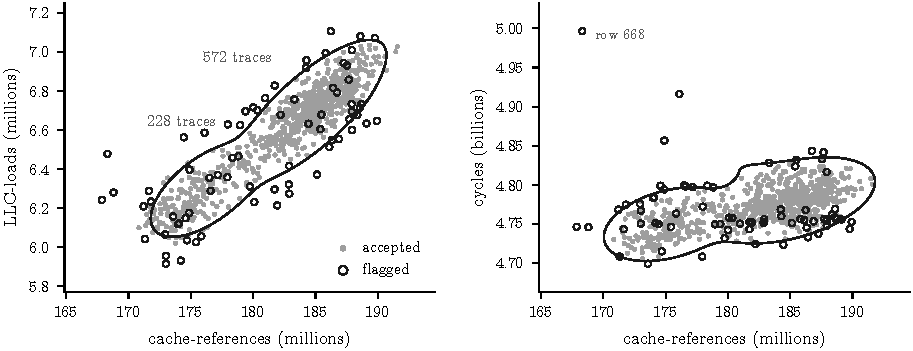
\includegraphics[width=\textwidth]{figures/fig_data.pdf}
  \caption{Clean training traces and the boundary of the region the final detector accepts. Left: LLC-loads
  against cache-references, with cycles at its median. Right: cycles against cache-references, with LLC-loads on
  its regression line. Open circles are the 72 training traces the detector flags.}
  \label{fig:data}
\end{figure}

\section{Detector}

We standardise the counters with the training mean and standard deviation and fit a Gaussian mixture with
$K = 3$ components and full covariance matrices. The anomaly score of a trace $x$ is its negative log-density,
\[
  s(x) = -\log \sum_{k=1}^{3} \pi_k \, \mathcal{N}(x \mid \mu_k, \Sigma_k).
\]
Full covariances let each component follow the cache-references/LLC-loads line. A trace whose counters are each
plausible but break that relationship then gets a low density, as does a trace that is extreme in one counter. The
fitted components hold 559, 219 and 22 training traces. The first two are the groups in Figure~\ref{fig:data}. The
third is wide and has a weight of 4\%. It covers the scattered traces around them.

To set the threshold we split the 800 traces into ten folds, fit the model on nine and score the tenth, which
gives one out-of-sample score per trace. The threshold is the $\lceil (n+1)(1-\alpha) \rceil$-th smallest of these
scores, the quantile used in split-conformal prediction~\cite{angelopoulos2021}. For a single calibration split,
it guarantees a false-positive rate of at most $\alpha$ on new clean traces from the same distribution. With
cross-fitting and a final refit on all 800 traces the guarantee is approximate, and in our repeated splits the
measured rate stayed between 0.038 and 0.058 for $\alpha = 0.05$. With $\alpha = 0.10$ the threshold is 4.664.

\section{Choosing the model}

Without backdoor traces we cannot measure detection rates on our own data, so we compared models in three ways.
\begin{enumerate}
  \item Clean false-positive rate on 20 random splits into 60\% fit, 20\% calibration and 20\% test, with every
        learned step fitted on the fit part only.
  \item AUROC against synthetic shifts. We moved held-out clean traces by 0.5 to 3 standard deviations along five
        directions: each counter alone, all three together, and the low-variance direction that breaks the
        cache-references/LLC-loads relation. These are guesses about what a backdoor might do, not attacks.
  \item AUROC on real backdoor traces from Alam et al.~\cite{alam2024}: 10\,000 clean and 10\,000 backdoor
        ResNet-18 inferences on an Intel i7-9700, with five counters, of which only cache-references matches
        ours. We fit on 640 clean traces to match our sample size.
\end{enumerate}

Table~\ref{tab:models} has the results. Every model kept its clean false-positive rate close to the target, so the
calibration works whatever the model. The synthetic shifts barely separate the models: most land between 0.83 and
0.86. The real backdoor traces do separate them (Figure~\ref{fig:auroc}). Their clean data also contains several
groups, and the z-score, Mahalanobis distance, PCA residual, one-class SVM and a one-component GMM all score
between 0.46 and 0.52. The mixture scores 0.81 with two components and 0.87 with three.

For the number of components we used held-out log-likelihood on our own data, from five-fold cross-validation
repeated four times: $-3.197$, $-3.004$, $-2.927$ and $-2.902$ for $K = 1$ to 4. BIC also prefers $K = 4$, but
its fourth component contains only the three cycle spikes, and a model that treats them as a group would accept
the next spike as normal. Against $K = 2$ on 40 identical splits, $K = 3$ had the higher held-out likelihood in
90\% of them and the same clean false-positive rate (0.051 against 0.048).

In a second round we tried a kernel density estimate with a cross-validated bandwidth, the mean distance to the
nearest clean traces, and an average of ten mixtures fitted on bootstrap samples. None beats the single mixture on
the real backdoor traces. Refitting the final model with eight different random seeds gave the same three
components each time and moved the threshold by $\pm 0.055$.

\begin{table}[t]
  \centering
  \small
  \begin{tabular}{lccc}
    \toprule
    Model & Clean FPR & Synthetic AUROC & AUROC, real backdoors \\
    \midrule
    z-score (largest $|z|$)              & 0.042 & 0.783 & 0.461 \\
    Per-counter GMM, as in \cite{alam2024} & 0.040 & 0.774 & 0.744 \\
    Mahalanobis distance (MCD)           & 0.052 & 0.828 & 0.521 \\
    PCA residual (2 components kept)     & 0.057 & 0.760 & 0.499 \\
    Isolation forest                     & 0.043 & 0.826 & 0.593 \\
    One-class SVM                        & 0.049 & 0.853 & 0.479 \\
    \midrule
    GMM, $K=1$                           & 0.046 & 0.848 & 0.497 \\
    GMM, $K=2$                           & 0.050 & 0.853 & 0.810 \\
    GMM, $K=3$ (final)                   & 0.049 & 0.858 & 0.865 \\
    \midrule
    Bagged GMM, $K=3$                    & 0.049 & 0.860 & 0.861 \\
    Kernel density                       & 0.047 & 0.842 & 0.793 \\
    5-nearest-neighbour distance         & 0.049 & 0.854 & 0.792 \\
    15-nearest-neighbour distance        & 0.048 & 0.853 & 0.761 \\
    \bottomrule
  \end{tabular}
  \caption{Model comparison. Clean FPR is the measured false-positive rate on held-out clean traces at a target
  of 0.05, averaged over 20 splits. Synthetic AUROC is averaged over five shift directions and four shift sizes.
  The last column uses the labelled traces of Alam et al., averaged over 10 splits.}
  \label{tab:models}
\end{table}

\section{Threshold}

AUROC depends only on how the scores rank traces, but the other four metrics depend on the threshold. In the
labelled traces a backdoor moves each counter by less than one clean standard deviation, so a strict threshold
misses most of them. Going from $\alpha = 0.05$ to $0.10$ raises TPR from 0.56 to 0.70, F1 from 0.69 to 0.77 and
accuracy from 0.756 to 0.797, at a false-positive rate of 0.11 (Figure~\ref{fig:alpha}). Beyond $\alpha = 0.10$
accuracy stops improving.

The best setting depends on how many backdoor traces the test set holds, which we do not know. Moving from
$\alpha = 0.05$ to $0.10$ improves accuracy only if at least about 30\% of the test traces are backdoored, or
40\% going by our synthetic shifts. We assumed a roughly balanced test set and used $\alpha = 0.10$. For a mostly
clean test set $\alpha = 0.05$ would be better. It is a single setting in \texttt{configs/final.json}.

\begin{figure}[t]
  \centering
  \begin{minipage}[t]{0.485\textwidth}
    \centering
    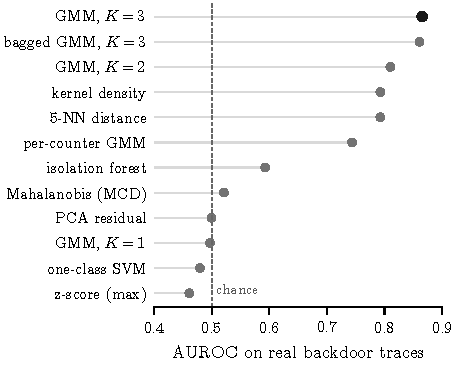
\includegraphics[width=\linewidth]{figures/fig_auroc.pdf}
    \caption{AUROC on the labelled traces of Alam et al.\ for each model.}
    \label{fig:auroc}
  \end{minipage}\hfill
  \begin{minipage}[t]{0.485\textwidth}
    \centering
    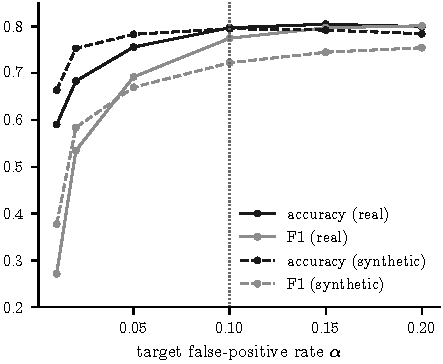
\includegraphics[width=\linewidth]{figures/fig_alpha.pdf}
    \caption{Accuracy and F1 of the final model as $\alpha$ changes, on the labelled traces (solid) and our
    synthetic shifts (dashed).}
    \label{fig:alpha}
  \end{minipage}
\end{figure}

\section{Limitations}
\label{sec:limits}

None of these numbers predicts our score on the hidden test set. The labelled traces of Alam et al.\ come from
other counters, a different CPU, a different network and a different trigger. We used them to compare methods,
not to estimate performance.

A detector trained only on clean traces cannot see a backdoor that leaves the counters where clean inputs already
put them, for example inside the other group. The hardest synthetic shift for our model was all three counters
rising together, with an AUROC of 0.79, against 0.93 for shifts that break the relation between cache-references
and LLC-loads.

In the data of Alam et al., traces from different recording sessions differ more than clean and backdoor traces
within one session. If the test traces were recorded in a different session from ours, the false-positive rate
could be higher than 10\%. And by construction about one clean trace in ten is flagged, so a flag means the trace
is unusual for a clean inference on these three counters, not that a backdoor has been proven.

\section{Code}

The detector is in \texttt{src/hpcdetect}. \texttt{scripts/predict.py} scores a new CSV with the saved model, and
\texttt{scripts/reproduce.sh} reruns every experiment, retrains the detector and rebuilds this report. All random
steps are seeded. The reference implementation of Alam et al.\ models each counter separately, sets its threshold
on the same traces it trained on, and removes outliers from the test data before scoring. We model the counters
jointly, calibrate on held-out traces and score every test trace as given.

\begin{thebibliography}{2}\small
\bibitem{alam2024}
M.~Alam, Y.~Wang and M.~Maniatakos.
\newblock Detecting backdoor attacks in black-box neural networks through hardware performance counters.
\newblock In \emph{Design, Automation and Test in Europe (DATE)}, 2024. doi:10.23919/DATE58400.2024.10546739.
Code and traces: \url{https://github.com/momalab/dnn-backdoor-detection-DATE24}.

\bibitem{angelopoulos2021}
A.~N. Angelopoulos and S.~Bates.
\newblock A gentle introduction to conformal prediction and distribution-free uncertainty quantification.
\newblock arXiv:2107.07511, 2021.
\end{thebibliography}

\end{document}
